%%
%% This is file `mcmthesis-demo.tex',
%% generated with the docstrip utility.
%%
%% The original source files were:
%%
%% mcmthesis.dtx  (with options: `demo')
%%
%% -----------------------------------
%%
%% This is a generated file.
%%
%% Copyright (C)
%%     2010 -- 2015 by Zhaoli
%%     2014 -- 2016 by Liam 
%%     2017 -- 2019 by Xuehan
%%
%% This work may be distributed and/or modified under the
%% conditions of the LaTeX Project Public License, either version 1.3
%% of this license or (at your option) any later version.
%%
%% This work has the LPPL maintenance status `maintained'.
%%
%% The Current Maintainer of this work is Xuehan.
%%
\documentclass{mcmthesis}
\mcmsetup{CTeX = false,   % 使用 CTeX 套装时,设置为 true
        tcn = 2102416, problem = C,
        sheet = true, titleinsheet = true, keywordsinsheet = true,
        titlepage = true}
\usepackage{palatino}
\usepackage{mwe}
\usepackage{graphicx}
%\usepackage{subcaption}
\usepackage{subfigure}
\usepackage{float}
\usepackage{multirow}
\usepackage{indentfirst}
\usepackage{gensymb}
\usepackage[ruled,lined,commentsnumbered]{algorithm2e}
\usepackage{diagbox}

\usepackage{geometry}
\graphicspath{{figure/}}
\geometry{left=2cm,right=2cm,top=2cm,bottom=2cm} %%页边距,若对左右边距进行修改,请保证左右边距一样,并且将mcmthesis.cls第81行对应的margin参数设置为相同数值
\begin{document}
\linespread{0.6} %%行间距
\setlength{\parskip}{0.5\baselineskip} %%段间距
\title{Buzz Receiving and Responding: Intelligent Report Classification Model}

\date{\today}
\begin{abstract}

 		Much attention has been attracted to Vespa mandarinia since they are first spotted in the USA in 2019. As the most savage alien insects, they pose a great threat to local agriculture and citizens' life. The State of Washington has encouraged the public to report sightings of these giant hornets while the correctness of reporting remains to be improved. In this paper, we construct an intelligent  report classification model based on automatic interpretation of reported files.
		
		\textbf{First}, as the premise of the model, we discuss the \textbf{predictability} of the spread of Asian giant hornets over time. Apart from proof from biology documents and existing models, we construct  \textbf{Scoring Probability Model (SPM)}  based on \textbf{distance} and \textbf{number of sightings} to testify that the spread is predictable. Level of precision is then calculated by estimating positive sightings among the unverified reports. The result is as low as  $22.22\%$, which calls for further improvement.
		
		\textbf{Second}, Computer Vision Process is operated on the data. We conduct data cleaning to the videos by intercepting the picture on each frame. Though the scale of given photos is \textbf{highly limited}, we extract the potential information to the fullest. Around 1100 photos are classified to \textbf{"Hornet-Like"} and \textbf{"Not-Hornet"} and over 600 photos are \textbf{labelled} by hand.After that, \textbf{LeNet framework Convolutional Neural Networks (CNN)} is utilized to operate \textbf{Similarity Matching}, then the result would be the similarity value.  We  then employ \textbf{YOLOv3} to do \textbf{object extraction algorithm} to examine  \textbf{the quality of a photo}. Both similarity value and quality of a photo constitute the score from image.
		
		\textbf{Third}, we conduct Natural Language Process to the notes. After stemming and lemmatization, words are transformed to vectors by \textbf{Word2vec}. \textbf{Similarity Matching} can thus be operated. We then combine \textbf{Characteristic Words Analysis} and \textbf{Sentimental Analysis} by constructing professional word set to quantitively interpret the sentences. The results of all three techniques make up the score from text.
		
		Our intelligent report classification model is \textbf{finally} built based on those two scores in combination with distance and time. The weight of each parameter is determined by \textbf{Analytic Hierarchy Process (AHP)}. We calculate the accuracy of the likelihood of a mistaken classification as $60\%$ and prioritize the submitted reports.
		
		As complement to the model, we determine the method and period of update taking  hornets reproduction model and citizens' habits into consideration. We thus build a detailed update pattern and a dynamic update period system based on \textbf{Difference Equation Model (DEM)} and public report submission frequency. Indication of the hornets eradication is provided as well.
		
		In conclusion, we build a  intelligent  report classification model by computer vision and natural language processing techniques. A complete update pattern and dynamic update period are given too. The classification model could predict the likelihood of a wrong classification within acceptable accuracy and prioritize the possible positive reports with high precision. The entire system could be used to enhance the prevention and control of the spread of Asian giant hornets in Washington.
	\begin{keywords}
	Intelligent Report Classification Model, Computer Vision, Natural Language Processing, Analytic Hierarchy Process, Difference Equation Model
	\end{keywords}
\end{abstract}

\maketitle

\tableofcontents
\newpage

\section{Introduction}
	\subsection{Background}
	Vespa mandarinia, also known as Asian giant hornet, is the largest species of hornet in the world. It has been spotted in Washington State since 2019 and caused a rush of panic over local authorities and citizens. These alien hornets are predators of other insects, especially  European honeybees which are pollinators of crops and vital to agriculture. It has been observed that a group of 20-30 Asian giant hornets kill 5,000-25,000 honeybees in a few hours \cite{intro0}. The economic loss is estimated to be more than 20 billion dollars if the land of North American is overrun by  Asian giant hornets \cite{intro1}. 
	
	In order to save local honeybees from the slaughter by Vespa mandarinia, the State of Washington has created certain channels for citizens to report sightings of these hornets. However, due to some inevitable reasons, the accuracy rate of public report is worrying. At the same time, additional investigation into possible presence of hornets requires  multitudes of official resources, which are extremely restricted. A new strategy utilized to prioritize these reports based on automatic interpretation of reported data is thus needed. Especially, several tasks are supposed to be completed:
	\begin{enumerate}
		\item a study and discussion of the predictability of the spread of Vespa mandarinia and its level of precision.
		\item a prediction model that  gives the likelihood of mistaken classification based on provided files and its discussion.
		\item a study of model update optimization in terms of update period. 
		\item a criterion of identifying the extinction of hornet based on the constructed model.
	\end{enumerate}
		
	Additionally, a two-page memorandum including all our results is required for the Washington State Department of Agriculture.

	\subsection{Our work}
		In this paper, we first validate the predictability of the spread. We then conduct data cleaning  to notes by stemming, lemmatizing and eliminating stopwords. Videos are processed through intercepting the picture on each frame as well. After that, we build our intelligent report classification model  based on four features: score from image, score from text, time and distance. Score from image is made up of similarity value and quality of the photo. These two parameters are analyzed by LeNet framework Convolutional Neural Networks (CNN) and YOLOv3 after 1100 photos are classified to "Hornet-Like" and "Not-Hornet" and 600 photos are labelled by hand. Score from text is determined by characteristic words analysis, sentimental analysis and similarity matching. The weight of each parameter in our classification model is then figured out by Analytic Hierarchy Process (AHP). In additional to the model, we construct a detailed update pattern including update period. Indication of the hornets eradication is finally provided. 

\section{Assumptions and Notation }
	First and foremost, some basic assumptions are made and their rationals are explained.
	\begin{enumerate}
		\item \textit{Citizens submit real data  in their report.}
		
		This is the premise of our work because our interpretation of data make sense only when the attached files like photos or notes are real.
	
		\item \textit{The nest of hornets is built in spring and abandoned in winter. It will not move during this time}
		
		It mainly bases on the provided background information to simplify our model \cite{intro0}.
		
		\begin{figure}[H]
	\centering
	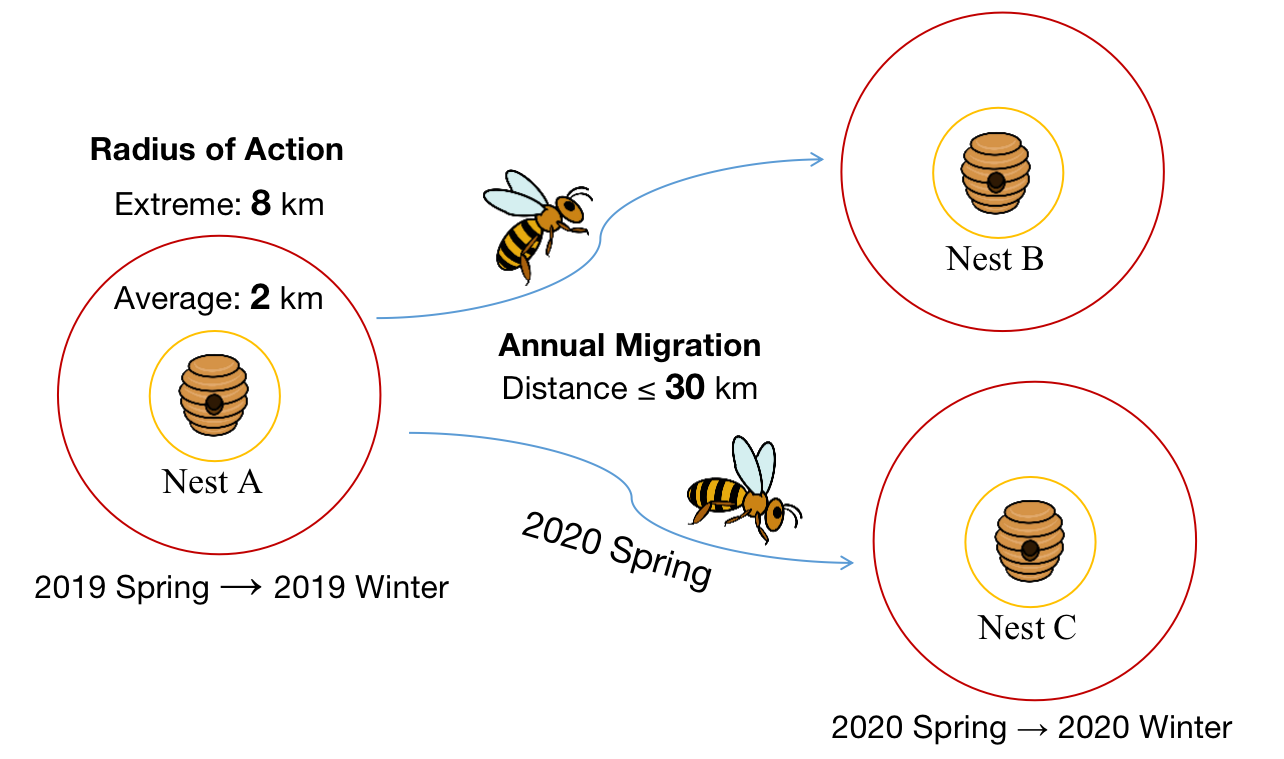
\includegraphics[width = 0.7\textwidth]{figure/assum.png} 
	\caption{Habits of Asian giant hornets involved in Assumption section}
	\label{fig:eg1}
\end{figure}
		
		\item \textit{The worker hornets could only be sighted within 8km from the nest. Also, the distance from any nest to the previous nest the same queen built is smaller than 30km.}
		
		This assumption is made according to Asian giant hornets' habits as shown in Figure \ref{fig:eg1} to avoid some extreme cases in our discussion \cite{intro0}.	
		
		\item \textit{The queen's cycle of birth only includes giving birth and raising the new-borns. That is to say,  the queen would give birth again immediately after finishing raising the latest new-borns.}
		
		This assumption bases on the Asian giant hornets' habits as well and is made to simplify the hornet reproduction model.
	\end{enumerate}
		


	Table \ref{tabbb1} contains the notations we use in this paper.

\linespread{1.2}		
		\begin{table}[H]
		\centering
		\caption{Notations \label{tabbb1}}
\begin{tabular}{c|c}
\hline
Symbol & Definition                 \\ \hline
$d$      & Distance                   \\
$k$      & Number of sights           \\
$I_1$     & Similarity with Hornets    \\
$I_2$     & Quality of Image           \\
$S_I$     & Score from Image           \\
$S_T$    & Score from Text            \\
$S_D$     & Score from Time Difference \\
$S_L$    & Score from Location        \\ 
$L$   & Likelihood Evaluation \\ \hline
\end{tabular}
\end{table}
\linespread{0.8}

\section{Task1: Predicting the spread of the pest}
	\subsection{Qualitative analysis}
	Much attention has been attracted to the quantitive modeling of spread of pests previously. To begin with, the life cycle of insects is highly regular and statistically satisfying, especially their reproduction period and immigration pattern \cite{reproduction}. Their spread tendency could be parametrized in the ideal conditions. Additionally, variety of mathematical methods have been utilized to model the spread of hornets in the past. Some results are consistent with observed data. For instance, Metropolis Hastings Markov Chain Monte Carlo (MCMC) method has been used in a Bayesian framework to construct prediction model \cite{Task_1_1}. It could simulate the spread and distribution of Vespa velutina (Asian hornet) in south-west France with acceptable precision \cite{Task_1_1}. In a word, due to hornets' regular life cycle and existing similar prediction models, the spread of  Asian giant hornets over time is predictable.
	\subsection{Scoring Probability Model (SPM)}
	\quad Now that the qualitative analysis of the prediction of the pest's spread is given in the previous part, quantitative analysis is conducted by introducing a scoring probability model (SPM). Since for this task, in order to show that the spread of the pest could be predicted, a quantitative method needs to provide a model with data provided and then its corresponding prediction as well as the precision. In the model we built, we make advantage of the positive sightings and divide it into two period: the positive sightings in 2019 and the positive sightings in 2020, and then we use them as the base of the prediction. Scoring probability model utilizes two factors of the reported sightings and then gives each reported place a score, the higher the score is, the more probable the sighting could be considered as positive. As for the two factors, one factor is the \textbf{distance} $d$ and the other is the \textbf{number of sightings} $k$ within certain areas. In order to determine these two factors, some related definition needs to be done: 
	\begin{enumerate}
		\item \textbf{Geometry center}\\
		First of all, geometry center is used to define the variable $d$. Since there exist 2 periods of the positive sightings, and based on the fact that "When winter arrives, the current seasons' nests die out", \textbf{the geometry center of the 2019 sightings are found and assumed as the origin} \cite{intro0}. Note that there are two extreme values in the 2019 sightings, we eliminate them to make the geometry center closer to most of the reported sightings to increase accuracy. Besides, the geometry center of the 2020 sightings are also found to compare the prediction results with the actual one.
		\item \textbf{The smallest cell}\\
		The smallest cell is used to define the variable $k$. In this case, the smallest cell refers to the smallest circle area we choose centered at each reported place, \textbf{the radius of the circle area is 2km}.	
	\end{enumerate}
	After we provide a proper definition of the geometry center and the smallest cell, the two factors could then be determined in the following ways, and in order to eliminate the dimensional influence between factors, \textbf{normalization} is also required to improve the comparability:
		\begin{enumerate}
		\item \textbf{distance} $d$\\
		Distance is determined by calculating the \textbf{straight distance} between the reported place and the geometry center of the 2019 positive sightings. Note that the straight distance here is calculated using the information of the \textbf{longitude and latitude} provided. The normalization is accomplished based on the following formula:
		\begin{align*}
			d_i = \frac{D_i-D_{min}}{D_{max}-D_{min}}, D_i \subset \text{Distance set} 
		\end{align*}
		where $D_{max}$ is the largest distance value and $D_{min}$ is the smallest.
		\item \textbf{Number of sightings} $k$ \\
		Number of sightings is determined by \textbf{the number of submitted reports} within the smallest cell centered at the reported place \textbf{over a year}. In the same way, the normalization is represented as follows:
			\begin{align*}
			k_i = \frac{K_i-K_{min}}{K_{max}-K_{min}}, K_i \subset \text{Frequency set} 
		\end{align*}
		where $K_{max}$ is the greatest number of sightings and $K_{min}$ is the smallest.
	\end{enumerate}
	In fact, based on the material, "A new queen has a range estimated at 30 km for establishing her nest", when the reported place is closer to the geometry center of the 2019 sightings, the greater the probability of the reported sighting being positive. As for the number of sightings, in order to eliminate the influence of over-reporting and zero-reporting, the mean value of 0 and 1, that is $\frac{1}{2}$ is chosen to be the base of the scoring function. Therefore, we apply the following function as our \textbf{scoring function} while the \textbf{input is the unverified data} provided, note that $\alpha$ here is a positive constant used to simplify other factors' effect:
	\begin{align}
		f(d,k) = \alpha*d*(\frac{1}{2})^{k}, \alpha > 0
	\end{align}
	\quad After obtaining Equation(1) as our scoring function, the number of the candidates needs to be settled to visualize the prediction of unverified data based on the scoring function. In order to manage this task, \textbf{frequency theory of probability} is applied as following: assume the probability of positive sightings equals the frequency of the positive sightings over the sum of positive sightings and negative sightings, given the exact number in the data, the candidate number is determined by the following formula:
	\begin{align*}
		number = \frac{12}{12+2069}\times 2342 = 13.5 
	\end{align*}
	since the number must be an integer, we round the result to 14 ($\pm 1$) as our final candidate number. The final prediction of the unverified data is presented in Figure \ref{marked} below.
	\begin{figure}[H]
		\centering
		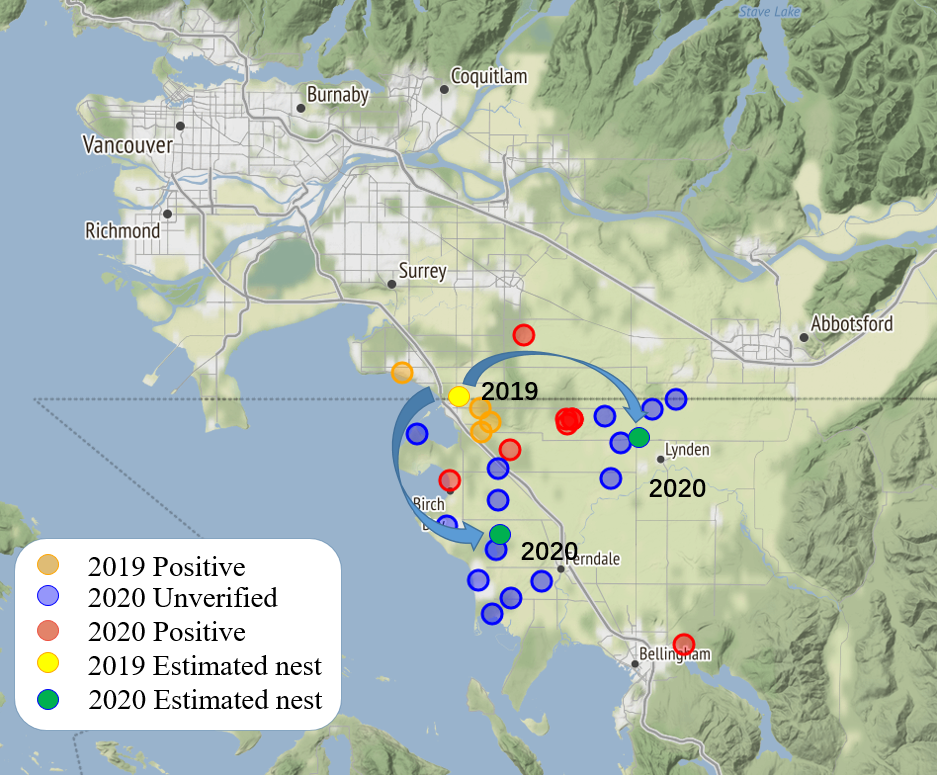
\includegraphics[scale=0.5]{marked.png}
		\caption{The prediction of unverified data}
		\label{marked}
	\end{figure}
	It could be seen on the figure that after we plot out the estimated nest (the geometry center) of the 2020 unverified reported sightings as well as the 2019 estimated nest (the geometry center of the 2019 positive sightings), the spread of the nest could be discovered. After we plot the arrows to indicate the direction of the spread, we found that it coincides with the fact that the Asian hornet originally "was discovered on Vancouver Island in British Columbia, Canada" since the nest of it has the tendency of coming down from the top to the bottom and invades the Washington state. In this way, the spread pattern and the prediction could be considered as predicted appropriately. Moreover, the precision of the prediction could be obtained based on the following scheme: The input data of the SPM is now not only the unverified data but also the positive sightings' data, since there are already 9 positive sightings in 2020, so we would choose 9 as the candidate number, and we take the coverage rate of the positive sightings based on the scoring function as the precision of the prediction:
	\begin{align*}
		Precision = \frac{n}{9}*100\%
	\end{align*}
	where $n$ is the number of positive sightings within top9 results ranked by the scoring function. Consequently, the precision is $\frac{2}{9}*100\%$ = \textbf{22.22\%} within $[20\%(\frac{2}{10}),25\%(\frac{2}{8})]$ (depending on the choice of candidate) since there are 2 positive sightings within the top9 results, and the result is presented in Figure \ref{marked2}.
	\begin{figure}[H]
		\centering
		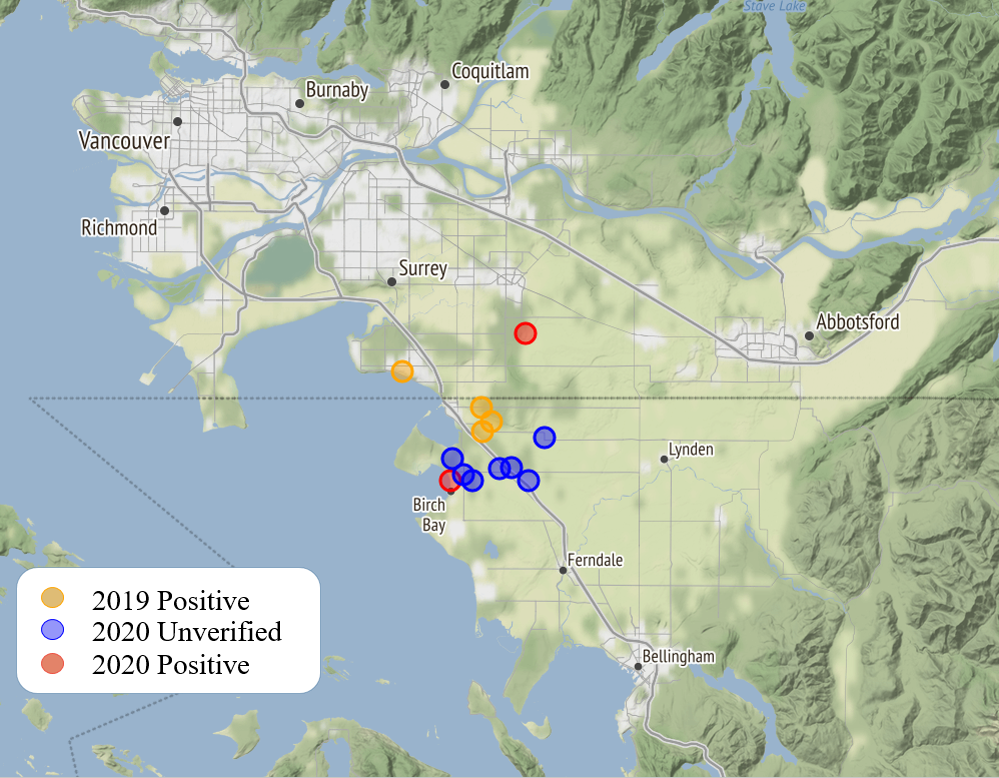
\includegraphics[scale=0.5]{marked2.png}
		\caption{The precision of the prediction}
		\label{marked2}
	\end{figure}
	
	Since the precision of the prediction is not accurate enough, further methods to provide a strategy to help the Washington state classify the submitted reports needs to be discovered, which would be shown in the next part.
	
	\section{Task2\&3: Intelligent report classification model}
	\quad Asian Hornets could be easily mistaken with other kind of hornets while tons of reports would flush right into the responsible department of Washington State, therefore, an intelligent report classification model is significant to be created in order to better inspect the pest's situation by giving the likelihood of reports' mistaken classification and quicken the process by prioritizing submitted reports at the same time. The flowchart (Figure\ref{flow}) below presents the whole creating process of the model.
	\begin{figure}[h]
		\centering
		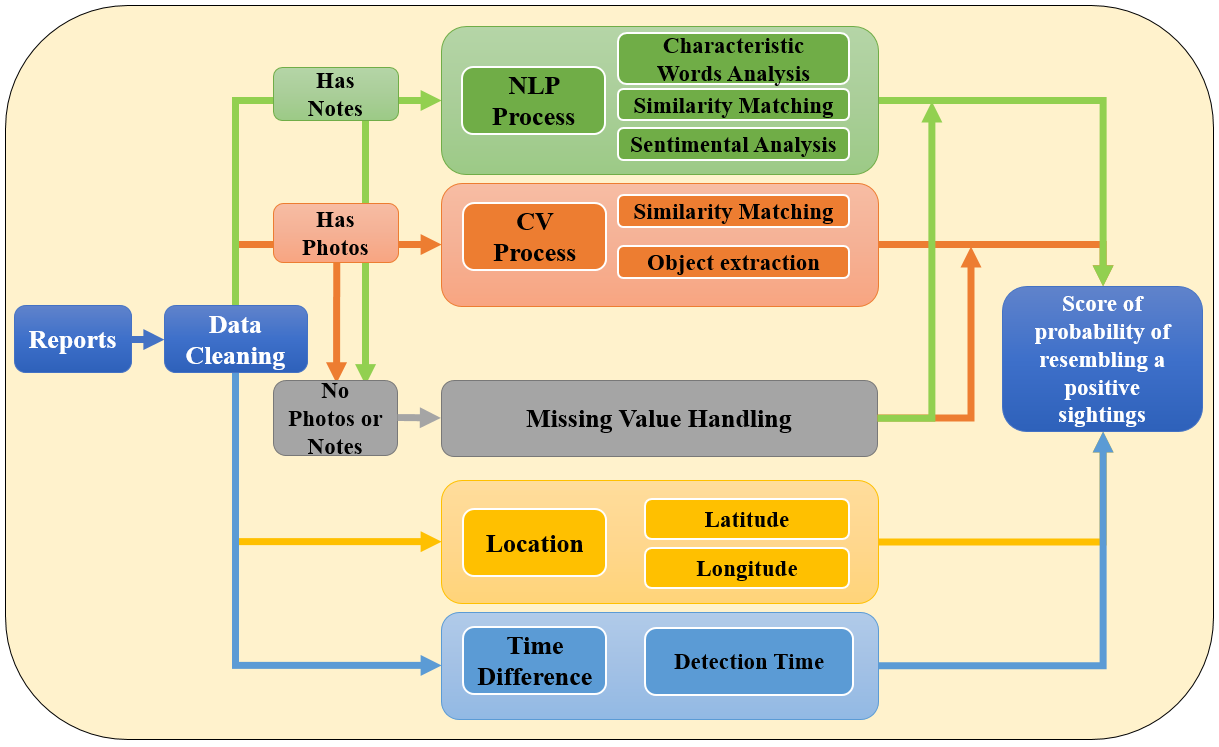
\includegraphics[scale=0.6]{flow.png}
		\caption{Flowchart}
		\label{flow}
	\end{figure}\\
	\subsection{Insight from the analysis of provided data}
	\quad From the provided data, it is obvious that \textbf{the sample of positive sightings are less than the negative sightings in a large scale (Positive: Negative = 14:2069)}, however, to create an intelligent model that could manage the task of providing effective classification requires us to make advantage of what we possess without extra information. As a result, coming up with \textbf{a way to weigh the validness of the information from reports is extremely important} to this task. What's more, we notice that there are a great deals of reports that lack one or several kinds of information such as reports without photos or reports without notes. Therefore, \textbf{how to process these outliers} is also important. After developing a way to solve these two major problems, \textbf{scoring evaluation} is adopted to make better predictions.
	\subsection{Weighing the validness of Image}
	\quad Information extracted from the provided data includes both image information and text information, so first of all, the following steps are the procedure of how we weigh the validness of the provided images and provide a single normalized score from the part of image.
		\subsubsection{Similarity matching applying CNN}
		\quad Similarity matching is one of effective ways to weigh the validness of images and given the fact that there exists shortage of the images from positive sightings, we decide to take a step behind and \textbf{change our target from matching Asian Hornets into the similarity matching built to match Hornets}. Before we put the similarity matching into practice, we first \textbf{label over 1100 provided photos into two kinds: "Hornet-Like" and "Not-Hornet"}. Note that "Hornet-Like" here represents the images that are comparably similar to the appearance of hornet and "Not-Hornet" here represents the images that have comparably great difference to the appearance of hornet including images that have no insects or other insects such as bee or beetles. In order to quantify the similarity we assign the value 1 to the image most "Hornet-Like" and 0 to the image most "Not-Hornet", which means the \textbf{final similarity value} for a single picture lies in the interval \textbf{[0,1)}. After labeling the photos, we apply \textbf{LeNet} framework Convolutional Neural Networks (CNN) to obtain the similarity value so as to weigh the validness of an image. Applying LeNet framework enables us to take an image as the input and obtaining the similarity output after several convolution layers and fully-connected layers \cite{LeNet}. The following figure Figure\ref{net} is the exact mechanism of the LeNet we applied.\\
		\begin{figure}[h]
			\centering
			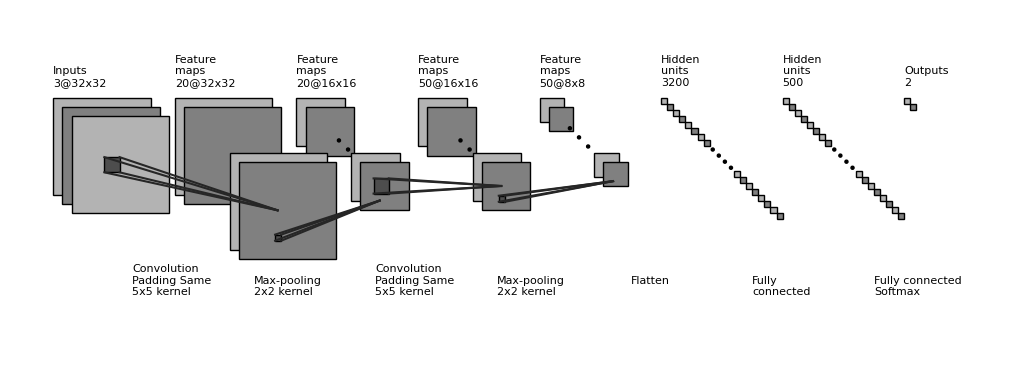
\includegraphics[scale=0.6]{net.png}
			\caption{Mechanism of LeNet}
			\label{net}
		\end{figure}
		\quad To evaluate the precision of the network we applied, Figure\ref{matrix} presents the \textbf{confusion matrix} generated according to the output of our LeNet framework. From the confusion matrix, we could calculate the precision of the output based on the number of the sample shown on the figure:
		\begin{align*}
			(712+410) \div (712+410+5) \times 100\% = \text{\textbf{99.5\%}}.
		\end{align*} 
	\begin{figure}[h]
   \centering
   \includegraphics[scale=0.45]{Matrix2.png}
   \caption{Confusion Matrix}
   \label{matrix}
  \end{figure}\\
		\subsubsection{Object extraction algorithm using YOLOv3}
		\quad The \textbf{quality of image} is another alternative that could be regarded as the standard to determine the validness of an image. Apart from the application of CNN, object extraction algorithm is also applied to weigh the validness of images.\textbf{YOLOv3} is one of the object extraction algorithm that has been applied to various regions of computer vision  \cite{Yolo}. As for our model, YOLOv3 is used to determine the quality of the image by locking down the part of the image that contains hornet and calculates the ratio of that part over the whole image which also stays in [0,1). Figure \ref{yolo} is an example of the result of the YOLOv3 algorithm we applied in our model. The quality of the image would also be included when scoring the validness of the image along with the similarity matching result.
			\begin{figure}[h]
			\centering
			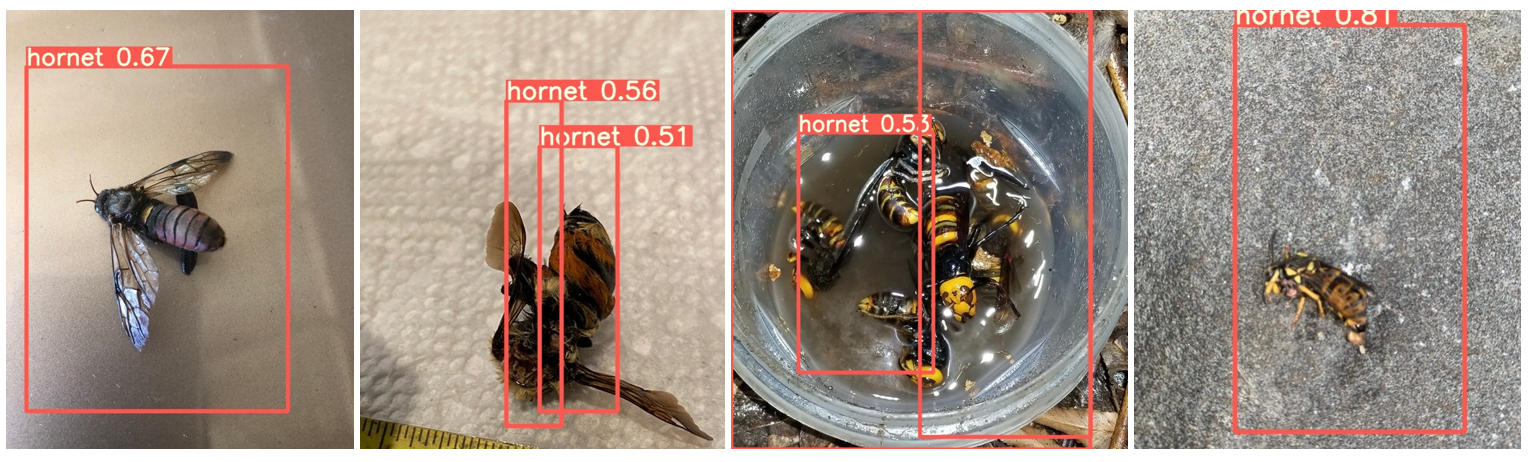
\includegraphics[scale=0.38]{yolo.png}
			\caption{Object extraction}
			\label{yolo}
		\end{figure}\\
		\subsubsection{Score from image}
		\quad As mentioned above, we now have two values $I_1$ from the similarity matching representing the similarity with hornet and $I_2$ as the quality of the image. In order to handle the \textbf{outliers} of image data, we assign \textbf{0.5} as the value of $S_I$ for them since a report without image could not be considered as purely negative or purely positive and 0.5 is the mean value of 0 and 1. This assignment \textbf{prevents the model to over score the reports with image data and completely ignore those without images}. We now take the function below as the scoring function of our model. The reason why we ignore the score coming from the quality of the image if $I_1\geq0.7$ or  $I_1\leq0.3$ is that after certain observation of the result, we found that if $I_1$ satisfies either the condition above, the quality score won't have much influence on the images' validness score.
	   \[S_{I}=\left\{\begin{array}{ll}
		I_1&I_1\geq0.7 \text{\space or\space} I_1\leq0.3,\\
		I_1 + 0.1I_2&
		0.3< I_1 < 0.7
	   \end{array}\right.\]
   	Note that we take the \textbf{maximum} score as the final score if there are multiple photos in a single reports.
	\subsection{Weighing the validness of Text}
	\quad In addition to the images provided, text worth a great deal to the intelligent classification model as well, and this is when natural language processing (NLP) comes into practice. The following steps are the procedure of weighing the validness of the text (mainly the \textbf{notes}) provided.
	\subsubsection{Characteristic words analysis}
	\quad As we all know, text consists of words, so we decide to \textbf{break down each sentence to words} from the notes and try to find a way to weigh their validness. To accomplish this goal, we first select several characteristic words describing the features of Asian Hornet from the authority article about the background information of Vespa mandarina provided. We also select some words that express the confidence of the reported person including the positive ones like "absolutely" and the negative ones like "unsure". Then we gather them into a set made up of characteristic words, after the set is created, we would match a sentence with the words in the set to score it. Note that we set the scoring amplitude of the positive confidence words less than the negative ones on account of the judgement of a normal person (not an expert on insects). If a person were confident about their positive judgement, the gap between their judgement and the fact are bigger than the one if there were negative about the results based on their own knowledge. The sample scoring mechanism is shown in Table\ref{words}.
	\begin{table}[h]
		\centering
		\begin{tabular}{ccc}
			\toprule
			Category &Word list &Score \\
			\midrule 
			Feature&yellow, orange, yellowish, black, giant, huge, big, large, strip $\dots$ &0.5\\
			Confirm&sure, confident, certainly, definitely, absolutely, without a doubt $\dots$ &0.2\\
			Suspect&not sure, unsure, doubt, possible, possibly, suspect, maybe  $\dots$ &-0.5\\
			\bottomrule
		\end{tabular}
		\caption{Sample scoring mechanism of characteristic words}
		\label{words}
	\end{table}
	\subsubsection{Similarity matching}
	\quad Not only the validness of the image could be weighed by similarity matching but the text as well. In this part, we first break sentences into words, and words could be represented by \textbf{vectors} (word-vectors) after going through the data-cleaning using "\textbf{word2vec}" algorithm, moreover we define the sentence-vectors as the \textbf{average value of the word-vectors in this sentence} \cite{Word}. Afterwards, \textbf{the semantic similarity between sentences could be represented by the similarity between sentence-vectors}. Now we just have to select several effective sentences in the notes to form an "\textbf{effective-sentence set}" as comparison. And we compare a sentence with every effective-sentence in the set to calculate the score. The pseudocode of this part is shown below.\\
	\begin{algorithm}[t]
		\caption{Weighing the validness of notes by similarity}
		\label{algo:event}
		\LinesNumbered
		\KwIn{The complete set of words used in notes $W=W_1,W_2,\dots,W_k$; The complete set of notes $U=U_1,U_2,\dots,U_n$, where $U_i \subset W \left(i \in \left[1,n\right]\right)$;The manual-defined set of valid notes $T=T_1,T_2,\dots,T_m$ and $T \subset U$}
		% \textbf{Require: } \
		\KwOut{The set of validness for each note $V$}
		{
			$W' \leftarrow$ \emph{Embedding $U$ by word2vec method and $W'$ is one to one mapping with $W$ by $f$};\
			$W'=W'_1,W'_2,\dots,W'_k$, where $W'_i \in R^{40}\left(i \in \left[1,k\right]\right)$ and $W'_i=f(W_i)$ \\
			% $W'= f(W)$. $$ \\
		}
		$X,Y \leftarrow$ \emph{Calculate sentence vector $X_i$,$Y_j$ for $U_i$ and $T_j$, where $U_i \in U$ and $T_j \in T$}; \
		$X \leftarrow X_i= \frac{1}{t} \sum_{p=1}^{t} f(w_p) (w_p \in U_i)$;\
		$Y \leftarrow Y_j= \frac{1}{t} \sum_{q=1}^{t} f(w_q) (w_q \in T_j)$
		
		\For{i $\leftarrow$ 1 \KwTo n}{	
			$V_i \leftarrow \frac{1}{m} \sum_{j=1}^{m}  CosineSimilarity(X_i,Y_j)$
		}
			\end{algorithm}
	\quad The scoring mechanism takes cosine similarity value as the similarity score, which is described as follows:
	\begin{align*}
		\text { similarity }=\cos (\theta)=\frac{A \cdot B}{\|A\|\|B\|}=\frac{\sum_{i=1}^{n} A_{i} \times B_{i}}{\sqrt{\sum_{i=1}^{n}\left(A_{i}\right)^{2}} \times \sqrt{\sum_{i=1}^{n}\left(B_{i}\right)^{2}}}\\
	\end{align*} 
	where $A,B$ are both sentence-vectors and $A_i,B_i$ represents the $i^{th}$ dimension value of $A,B$. Finally we take the \textbf{average value as the score of the sentence}.
	\subsubsection{Sentimental analysis}
	\quad When discussing about text, sentimental analysis is always a way to weigh the validness. In this case, we use the "\textbf{textblob}" package in python to manage the job, and the final score lies in the interval [0,1], where 0 represents absolute subjective tones and 1 represents absolute objective tones. The score of the sentimental analysis would be added to the final score as well as the previous two scores.
	\subsubsection{Score from text}
	\quad As mentioned above, we now have $T_1,T_2,T_3$ coming from the  Characteristic words analysis, similarity matching and sentimental analysis. scores to weigh the validness of text.Since we want to enlarge the difference between the "negative text" and positive ones in order to make the score more appropriate, multiplying $T_1$ and $T_2$ is an option, for example, suppose $T_1 = 0.1,T_2=0.1$, if we simply add them the result would be 0.2 instead of 0.01 gained from multiplying. The following is the scoring function combing all three of them:
	\begin{align*}
		S_T = T_1*T_2+T_3
	\end{align*}
    \subsection{Score from location and time difference}
    \quad Location of the submitted report and time difference is considered in the model as well. For the score of location, we first find out the location of the submitted report and calculate the distance between it and the \textbf{nearest positive sighting's location}, the nearer the distance, the higher the score $S_L$ is. As for the score of time difference, it works in the same way: we find out the detection time of the report and calculate the time difference between it and the \textbf{latest positive sighting's time}, the smaller the difference, the higher the score $S_D$ is.After we perform \textbf{normalization}, both of the scores stay in the interval of \textbf{[0,1]}.
	\subsection{Evaluation with AHP}
	\quad Analytic Hierarchy Process (AHP) is often used to evaluate a multi-factor model and set the weight of each factors. In this case, our AHP hierarchy is demonstrated as Figure\ref{AHP}:\\
	\begin{figure}[h]
		\centering
		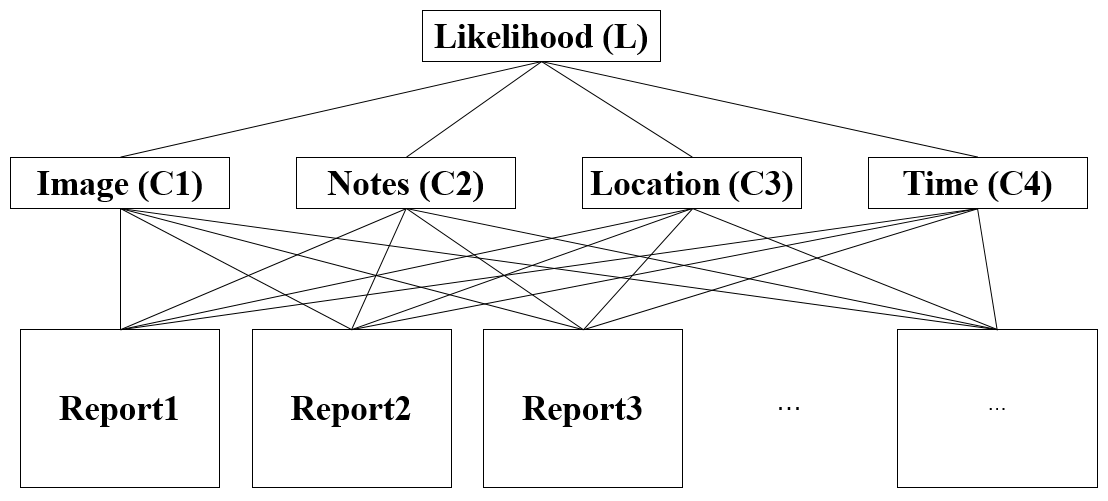
\includegraphics[scale=0.5]{AHP.png}
		\caption{AHP hierarchy}
		\label{AHP}
	\end{figure}
	Note that the likelihood here stands for the \textbf{probability of resembling a positive sighting}. The pairwise comparison matrix is given as follows:\\
	\begin{figure}[H]
		\centering
		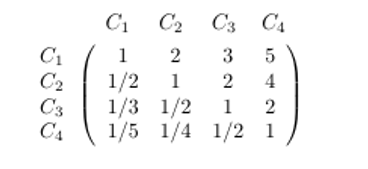
\includegraphics[scale=0.8]{m.png}
	\end{figure}
	Thus we have the \textbf{evaluation (scoring) function} shown as Equation\ref{score}, in which coefficients $\omega_1,\omega_2,\omega_3,\omega_4$ to be determined:
	\begin{align}
		L = \omega_1S_I + \omega_2S_T + \omega_3S_L + \omega_4S_{D}
		\label{score}
	\end{align}
	where $S_I,S_T,S_L,S_D$ are the normalized scores corresponding image, text, location and time difference. After calculating, we obtain the values of these coeffcients: $\omega_1 = 0.4772,\omega_2 = 0.2880,\omega_3 = 0.1539,\omega_4 = 0.0809$. Then we need to perform the following consistency test to the results we get:
	\begin{enumerate}
		\item \textbf{The test of consistency index $CI$}\\
		\begin{align*}
			CI = \frac{\lambda_{max}-n}{n-1} = \frac{4.0211-4}{4-1} = 0.0070
		\end{align*}
	which is very \textbf{close to zero}.
		\item \textbf{The test of consistency ratio $CR$}\\
		\begin{align*}
			CR = \frac{CI}{RI} = \frac{0.0070}{1.2} = 0.0078
		\end{align*}
	where $RI$ is the corresponding random consistency index when $n=4$, and the result 0.0078 is less than 0.1.
	\end{enumerate}
	Therefore, these coefficients pass the consistency test perfectly, and the final scoring function would be as follows:
	\begin{align}
		L = 0.4772S_I + 0.2880S_T + 0.1539S_L + 0.0809S_D
		\label{final}
	\end{align}
	\section{Model Application}
	\subsection{Task2: Likelihood of the mistaken classification}
	\quad In Task2, we need to determine the likelihood of the mistaken classification, the first thing of all is to \textbf{evaluate every report and rank them} using Equation\ref{final}. Then based on the fact that there are about half of the reports rated as "negative sightings" in the provided data, we select the last 50\% from the rank that has lower scores and calculate \textbf{the ratio of "negative sightings" over half the reports number}:
	\begin{align*}
		\text{Likelihood} = \frac{1337}{2220}
		\times 100\% = 60.2\% 
	\end{align*}
	since there are overall 4441 reports.Thus, the likelihood of the mistaken classification would be \textbf{60.2\% $\pm 0.01$\%} (uncertainty calculated by using 2219 and 2221 since we have rounded the result to be an integer 2020), which is also demonstrated in Figure\ref{t2}.
	\begin{figure}[h]
		\centering
		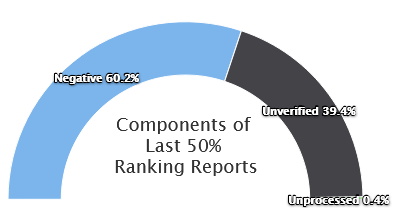
\includegraphics[scale=0.85]{task2.png}
		\caption{Components  of last 50\% ranking reports}
		\label{t2}
	\end{figure}
	\subsection{Task3: Prioritizing submitted reports}
	\quad As for Task3, we need to prioritizing submitted reports that most likely to be positive sightings, the intelligent classification model already provide the scores of them, representing the likelihood of being "positive sightings", which means the higher the score, the more likely to be positive, and this leads to "firstly investigated". Therefore, since the input number of reports could be large, we \textbf{choose the top 5\% of the reports based on their rank after applying the evaluation function} to be examined in priority. The precision of the prioritizing process could be tested in the following way: we apply the scoring function to the 4441 reports provided and choose the top 5\%, since there are only 14 positive sightings, the precision would be the ratio of "positive sightings in the rank top 5\%" over 14:
	\begin{align*}
	\text{Precision} = 11\div14 \times 100\% = 78.6\%
	\end{align*} 
	and the exact details are presented in Figure\ref{t3}.
	\begin{figure}[h]
		\centering
		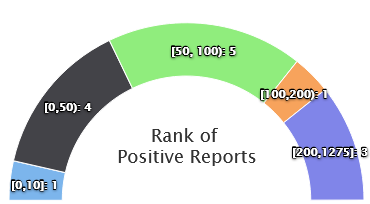
\includegraphics[scale=0.85]{task3.png}
		\caption{Rank of positive reports}
		\label{t3}
	\end{figure}
	\subsection{Overall evaluation of the model}
	\quad To evaluate the overall performance of our model, t-SNE is used to reduce the dimension to a 2-dimensional space and visualize the results, which is shown in Figure\ref{tsne}. It could be seen from the figure that the all the reports could be divided into 3 parts. From left to right, the likelihood of the reports to be considered as "positive sightings" increases. \textbf{The clear boundary between each 2 parts demonstrates the success of the classification based on the evaluation function.}
	\begin{figure}[h]
		\centering
		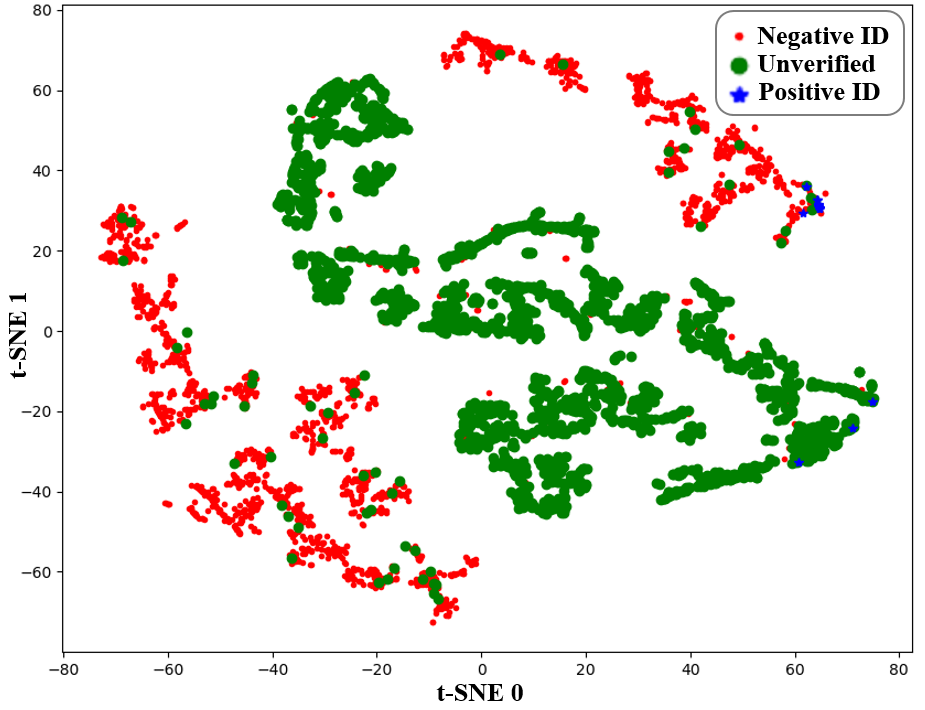
\includegraphics[scale=0.6]{TSNE.png}
		\caption{t-SNE: Overall performance}
		\label{tsne}
	\end{figure}
\section{Task4: Update of the model}
	\quad A well-rounded model is said to be developing if it follows the trend and updates itself after certain periods. To update the model we have built, both the method and frequency of the update should be covered, which we would make a demonstration in this task.
	\subsection{Method of the update}
	\quad As for the method to update our model, because our model includes Computer Vision (CV)), Natural Language Processing (NLP) as well as the location and time difference of the reports, the update should cover them all as well. Suppose the model needs to be updated after a while, and we now possess certain amount of reports data, the following is the update procedure:
	\begin{enumerate}
		\item \textbf{Update the photos (Include videos)}\\
		Among all the reports, the photos attached in the report could a great use. If it were videos, in the same way, we extract the keyframe and treat it as photos. Based on the mechanism of our model, the photos require labelling, so after obtaining all the photos we label them and try to make classification afterwards, which means we sort out some comparably clear photos containing hornets. Then we gather all the \textbf{"well-being" photos and put them in the training set} we have already created and use them to train other image data.
		\item \textbf{Update the notes in the reports}\\
		Notes in the reports could be processed in the same way with the photos. We classified them and select some \textbf{valuable comments} which have detailed description of the hornets. Then we \textbf{insert them in the database} of our NLP training set and use them for classifying. 
		\item \textbf{Update the location and time difference}\\
		As for the final step, we update the location and the time difference of the reports and insert them in the database for further intelligent classification.
	\end{enumerate}
	\subsection{Frequency of the update}
	\quad After understanding how to update the model given additional new reports over time, deciding how often the model should be updated is the next request to be tackled. In order to help Washington State better supervise the growth of the Asian Hornet and investigate the efficiency of the pest control, both the \textbf{population growth of the Asian Hornet and the submission frequency of the reports over a year} should be taken into account.
	\subsubsection{Difference Equation Model (DEM)}
	\quad Since the analysis of the Asian Hornet's population growth is necessary for this task, it is essential to observe the curve of the population growth before giving the strategy of the update frequency. It is universally acknowledged that Asian Hornet could be classified into a bigger group-insects, and all insects' population growth have certain patterns. Based on the fact that "only the queens could give birth" and "the nest would die out in winter and only the queen would survive", we could assume that the population growth of the Asian Hornet belongs to the region of \textbf{discrete growth} since there exist special individual that only it could give birth to new life and the duration of the life cycle is counted by year \cite{intro0}. To simplify the model, we assume that the queen's cycle of birth only includes giving birth and raising the new-borns, which means the queen would give birth again immediately after finishing raising the latest new-borns. Therefore, \textbf{difference equation model (DEM)} is applied to investigate the population growth of the Asian Hornets:
	\begin{align}
		N_{t+1} = N_{t}f(N_t)
		\label{epm1}
	\end{align}
	 Note that $N_t$ here is the population of the t$^{th}$ generation, and t$^{th}$ generation could be simply defined as the Asian Hornets that are born and raised in the t$^{th}$ cycle of birth. Being a part of the insects, Asian Hornets's population would also be affected by the \textbf{Crowding Effect}, which illustrates the idea of the decrease of the population growth rate due to the large density of the species, the limited capacity of the nest or some other issues \cite{reproduction}. Consequently, suppose the peak population is $N_p$ and the growth rate would change by $B$ linearly depending on both $N_p$ and the current population, $f(N_t)$ could be rewritten as below \cite{reproduction}:
	 \begin{align*}
	 		\lambda = f(N_t) = 1-B(N_t-N_p)
	 \end{align*}
 	As a result, Equation\ref{epm1} now is in the form of:
 	\begin{align}
 		N_{t+1} = (1-B(N_t-N_p))N_{t}
 		\label{epm2}
 	\end{align}
 	which considers the influence of the crowding effect.
 	\subsubsection{Application of the DEM}
 	\quad In order to apply the DEM introduced above for our task, we need to use the initial condition to find the coefficient $B$ along with the final number of generation $t_{final}$ before plot the figure out. First of all, according to the fact that "the peak would be around 100 workers in August" and "up to 65\% of the queens not being fertilized", we estimate the \textbf{peak population} in the following way: Suppose there are 5 queens that are fertilized,
 	\begin{align*}
 		Original-Queens &= \frac{5}{35\%} = 14.285, \text{which rounds to 15 (integer)}\\
 		N_p &= 100 + 15 = 115
 	\end{align*}
 	The peak population number 115 here might stay in the interval [110,120] considering the effect of the males and queens as well as the workers. Afterwards, since the peak population appears in August and the nest begins growing at the start of Spring, we only examine the population growth \textbf{from March to August}. As for the final number of generation $t_{final}$, according to some related materials, the birth cycle of Asian Hornets is about 20 days, then we could estimate $t_{final}$ in the following way \cite{intro0}:
 	\begin{align*}
 	 t_{final} = \frac{31+30+31+30+31+31}{20} = 9.2,\text{which rounds to 9 (integer)}
 	\end{align*}
	 Up to now we have obtained the value of the peak population which is also the value of $N_{t_{final}} = N_9 $, and there is no doubt that $N_0 = 1$ since only the queens would survive the winter and start a new nest, we have obtain both the boundary value of the difference equation and if we combine the boundary values with based Equation\ref{epm2}, the equation of $B$ is now:
 	\begin{align*}
 		N_{t+1} = (1-B(N_t-N_p))N_{t},\text{\space} N_0 = 1,\text{\space} N_9 = N_p = 115
 	\end{align*}
 	The result of $B$ is $B = 0.00918$, and since we estimate it using $t_{final} = 9$, if we estimate it with $t_{final} = 10$, $B$ would become 0.00881 instead, in conclusion, $B$ belongs to the interval [0.00881,0.00918]. After obtaining the result of the coefficient $B$, Equation\ref{epm2} \textbf{the difference equation has the simplified form}:
 	\begin{align}
 			N_{t+1} = (1-0.00918(N_t-115))N_{t}
 			\label{eqm3}
 	\end{align}
 	\quad Using Equation\ref{eqm3} above, we plot the figure of the population growth of Asian Hornet from March to August, which is presented in Figure\ref{p}.
 	\begin{figure}[h]
 		\centering
 		\includegraphics[scale=0.5]{after.png}
 		\caption{Population growth of Asian Hornet}
 		\label{p}
 	\end{figure}
 	Frome the figure, we could notice that the growth rate would increase slowly at first and rapidly in the middle and then decrease when reaching the end, this could be utilized to \textbf{decide the frequency of the update of the model since the model needs to consider the growth rate of the Asian Hornets}.
 	\subsubsection{The influence of the submission frequency and decision of update frequency}
 	\quad As for now we are seeking for a model that could benefit the Washington State to sort out and prioritize the submitted reports for inspection of the pest, the influence of the submission frequency needs to be involved when deciding the frequency of the update. Figure \ref{f} below is the statistics of the number of the submission reports each month over a year.
 	\begin{figure}[h]
 		\centering
 		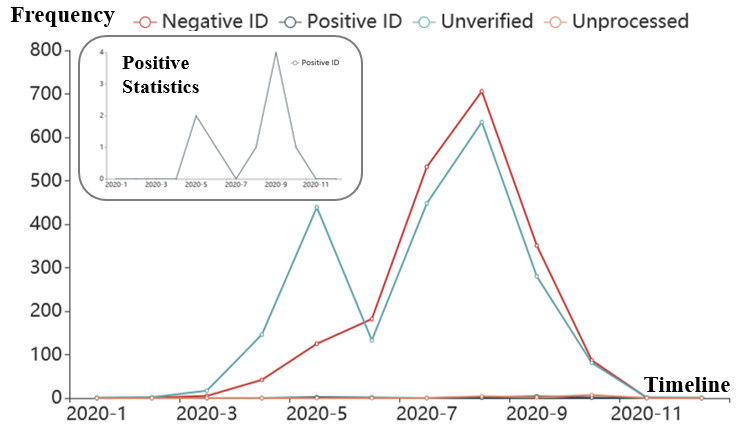
\includegraphics[scale=0.7]{f2.png}
 		\caption{Number of submission reports}
 		\label{f}
 	\end{figure}
 	From the figure, the tendency of the submission could be interpreted as follows: people tend to report sightings rapidly around August, which coincides with peak population and after August \textbf{the submission number drops nearly linearly due to the life cycle of the Asian after August and the almost reaches 0 approaching November}. Built to better help the Washington State handle the submission report, the model should consider both the input number of the report and the population growth of the Asian Hornet, and that's why we should \textbf{allocate the frequency of model's update dynamically}. The \textbf{scheme} is shown as below and visualized as Figure\ref{scheme}.

 	\begin{enumerate}
 		\item \textbf{Before August: Follow the growth rate of the population}\\
 		After analyzing the curve of the population growth rate, first few generations grow slowly and the growth rate increases rapidly in the middle part of a year and then slow down again. In order to follow the trend to inspect the growth of Asian Hornet, we could set 20 as the limit number and we update the model when the population increases by the amplitude of 20 each time before August. Based on the population growth curve, this means we \textbf{starts from March and update the model by 80 days (4 generations), 20 days (1 generations),20 days (1 generations), 10 days (half a generation),10 days (half a generation), 20 days (1 generations)  until the beginning of August.}
			\begin{figure}[h]
 		\centering
 		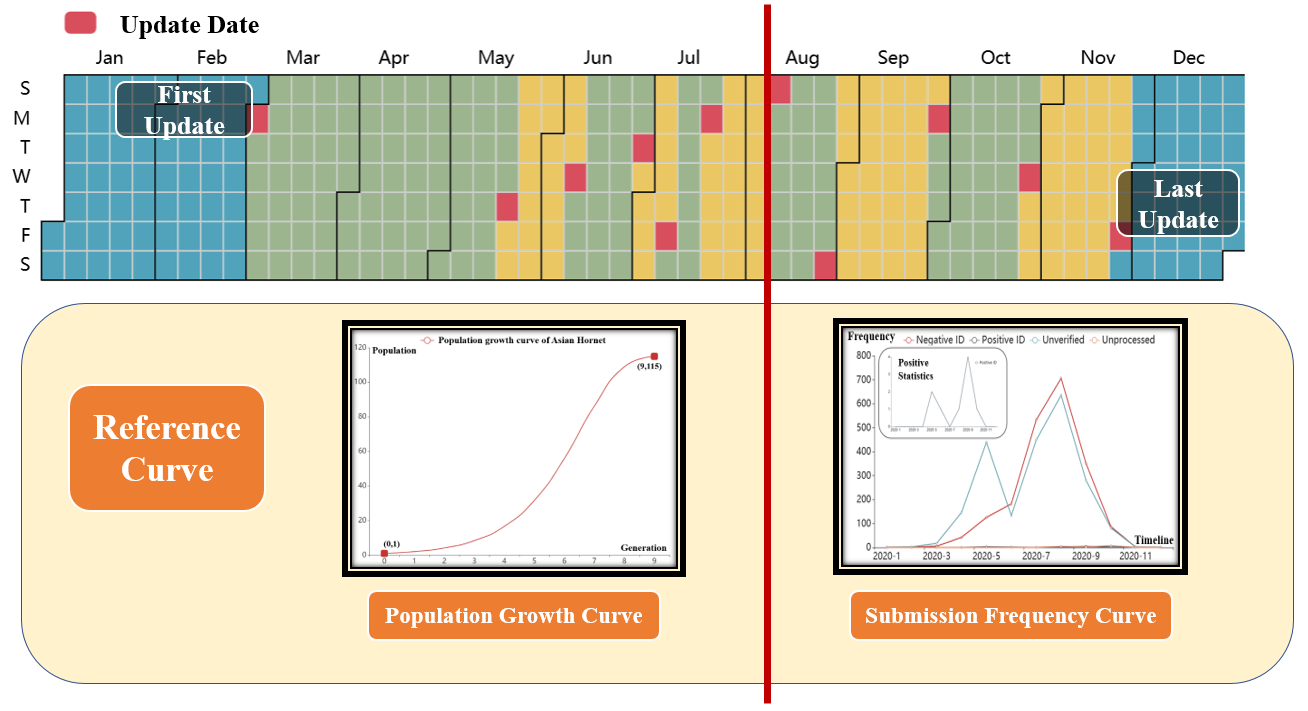
\includegraphics[scale=0.56]{scheme.png}
 		\caption{Update frequency scheme}
 		\label{scheme}
 	\end{figure}
 		\item \textbf{After August (Includes August): Follow the trend of the submission frequency}\\		
 		When time approaches August, the population reaches the peak, despite the declination of the growth rate, the submission reports frequency enlarges a great deal, which then creates a big gap of the input reports. As to deal with the large input number of the reports, we need to keeps the update time as 20 days (1 generations) to keep up the process and then slow down the process after August: \textbf{20 days (Beginning of August), 30 days (September-November), and from November to the end of February next year, we could stop updating} since most of the Asian Hornets die and the queens won't show up as well. 
 	\end{enumerate}
\section{Task5: Indication of the eradication}
	\quad Under the circumstances that Washington State tries to use the model to inspect the living condition of Asian Hornet, submitted reports would be the main source used to judge whether the pest is about to be extinct or not. In consequence, patterns of the reports or information extracted from the reports would constitute evidence that the pest has been eradicated in Washington State. Before introducing the judging strategy, the knowledge of the extinction of a certain species should be covered. In fact, a species could be considered as extinct if the following statement is satisfied: "although a small number of individuals of that species still exist, there are no reproducible individuals or there are only a small amount which is lower than the minimum limit for the existence and reproduction" \cite{functional_extinction}. That is, to estimate the minimum limit, we suppose there is only 1 queen left since only queen could give birth, then since "a large percentage of queens (up to 65\%) not being fertilized", we could allow $1 \div 0.35 = 2.8$ which rounds up to 3 queens within the estimate interval of [2,3] at the same time but still considered as extinct. Based on the model we built and the definition of extinction, the \textbf{judging strategy on the pest's extinction} is demonstrated as follows, which must \textbf{satisfy two statements}.The strategy focus on the inspection of the submitted reports in \textbf{Spring and Winter in the same year} since we could both handle the input number and the model has been updated:\\
	\begin{enumerate}
		\item \textbf{Spring}\\
			In \textbf{Spring( March or April}), the population starts to grow but not too large so that we could handle the input number properly. We could first sort out the reports that belong to "positive" or "unverified", then we use our model to prioritize the mostly likely positive sightings in "unverified" reports and mark them on the map. Then we follow task1's idea: we locate the nest of the Asian Hornet by enclosing the "positive sightings" with a circle whose radius is 30km (the maximum action radius of queen). Then we count \textbf{the number of the estimated nest}, if the value is \textbf{smaller than 3}, then it satisfies this statement, otherwise, it doesn't.
		\item \textbf{Winter}\\
			When time reaches \textbf{Winter( Late October or November)}, the number of submission starts to drop so we could better handle the input number as well. Besides, in Winter, the workers start to die and the queens start to migrate, so after we collect all the reports, we could still enclose the calculated "positive sightings" with a circle whose radius is 8km (the maximum action radius of worker), if \textbf{the number of the action circle} is \textbf{less than the number of the nest in Spring or even reaches 0 and shows a tendency of declining}, we consider it satisfies the requirements, otherwise, it doesn't. 
	\end{enumerate}
	The detailed demonstration of enclosing is shown in Figure\ref{circle} below.
	\begin{figure}[H]
		\centering
		\subfigure[30km-Enclosing]{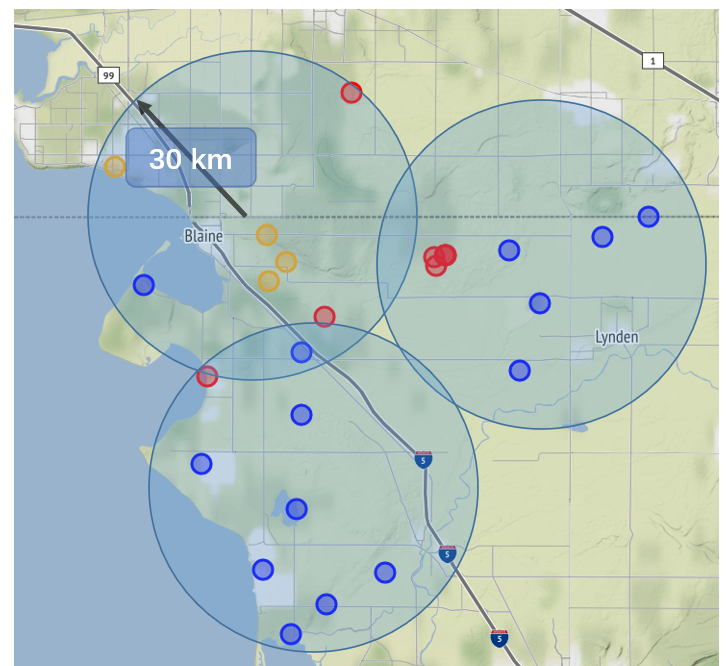
\includegraphics[scale=0.323]{1.png}}
		\subfigure[8km-Enclosing]{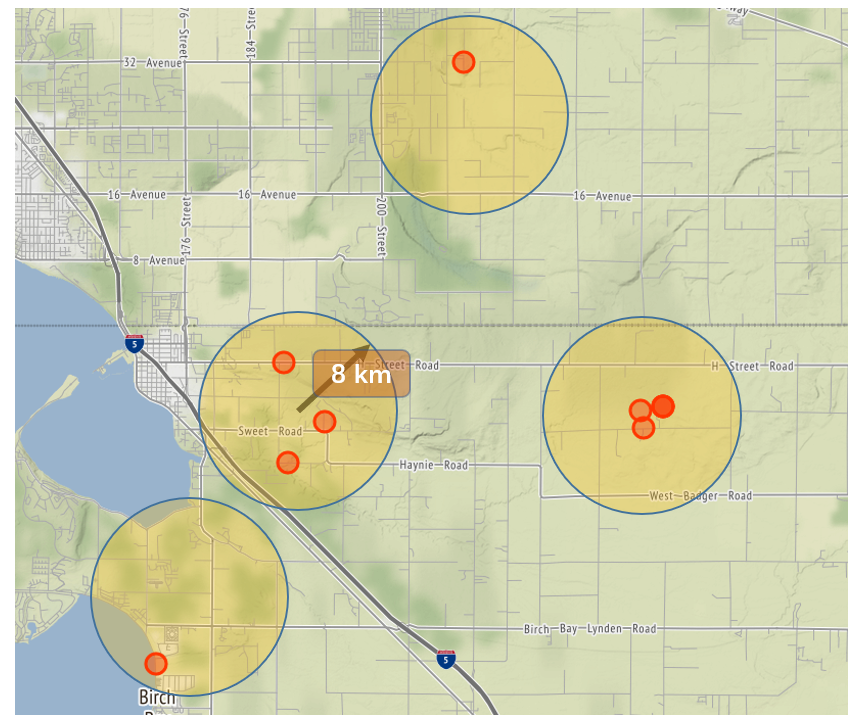
\includegraphics[scale=0.30]{2.png}}
		\caption{Mechanism of enclosing}
		\label{circle}
	\end{figure}
\newpage

\section{Sensitivity Analysis}
	We prose into the sensitivity of the ranking of the report in the prioritized list  and the likelihood of a mistaken classification. Since in our model, the factors of CV and NLP results counts a lot:
	\begin{equation*}
		L=0.4772 S_{I}+0.2880 S_{T}+0.1539 S_{L}+0.0809 S_{D}.
	\end{equation*}
	where $0.4772$ and $0.2880$ are the largest weights. Now we define $\Delta$ as the change of the value and the equation can be expressed as
	\begin{equation*}
		L=(0.4772-\Delta) S_{I}+(0.2880+\Delta) S_{T}+0.1539 S_{L}+0.0809 S_{D}.
	\end{equation*}
	
	Let $\Delta$ be assigned from $0$ to $0.3$, we calculated the score of each report based on our model and then prioritize them. To explore the influence of changed parameters, we picked all the reports with positive ID, as shown in Figure \ref{fig_sen1}.Note that in this figure, each curve represents the ranking of one report.
	\begin{figure}[h]
\begin{minipage}[t]{0.49\linewidth}	
\centering
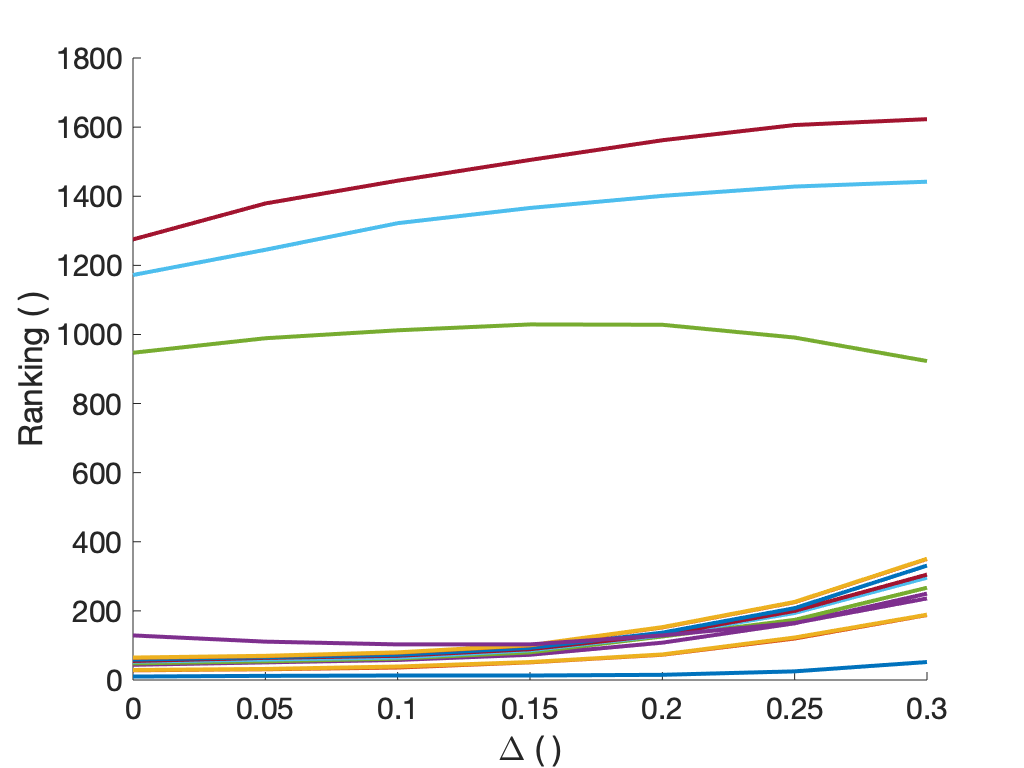
\includegraphics[width=1.1\textwidth]{sen1.png}	
\caption{Sensitivity of ranking \label{fig_sen1}}  
\end{minipage}
\hfill
\begin{minipage}[t]{0.5\linewidth}
\centering
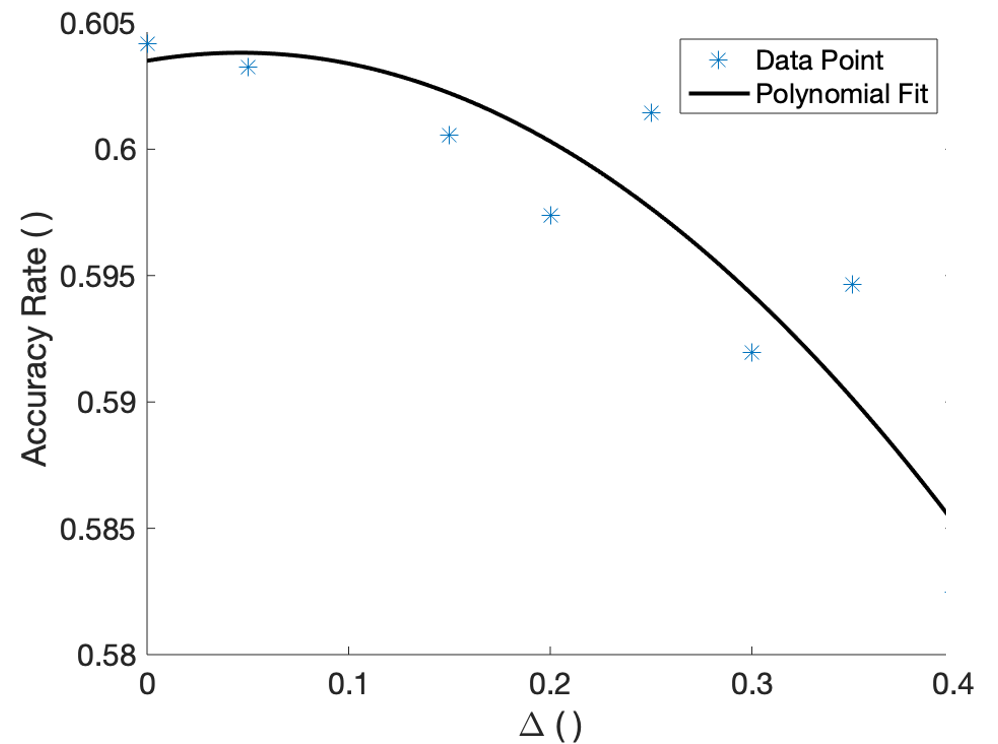
\includegraphics[width=1.1\textwidth]{sen2}
\caption{Sensitivity of likelihood\label{fig_sen2}}
\end{minipage}
\end{figure}
 
 It is clear that the ranking of report with positive ID tend to decrease as the weight of the score obtained. The change rate of the ranking, however, has been shown to be small. As   $\Delta$ approaches $0.3$, most of the reports with positive ID still rank high in the list----- $78\%$ in the top 400. Therefore, it is safe to conclude that the ranking of the reports in the prioritized list has low sensitivity.
 
 	Then we explore the sensitivity of the likelihood of a mistaken classification. The accuracy rate are figured out in the same way that used in Task 2.Also, we perform a polynomial fit to the result, as shown in Figure \label{fig_sen2}. The fitting function is 
	\begin{equation*}
		y = -0.1485 x^{2}+0.01375x+0.6035
	\end{equation*}
 	with adjusted $R^{2}$ of $0.8026$.

	It is displayed that the change of accuracy is fewer than $2\%$ even when the weight of CV parameter is reduced to around 0.1. The derivative of the fitting function is quite small as well. The robustness of the result is thus proved to be adequately strong.
\section{Strength and Weakness}
	\subsection{Strength}
		\begin{itemize}
			\item \textbf{High Precision:} the model could predict the likelihood of a mistaken classification with the accuracy of $60$\%. In addition, most reports with positive ID ($78$\%) ranked in top $200$ among over $4000$ reports on the prioritized list. Since the public is easy to muddle Asian giant hornets and local pests, it is a substantial improvement to the information classification and corresponding investigation.
			\item \textbf{Human-oriented Design:} the model could save multitudes of human resources. It automatically prioritizes the reports and gives the likelihood of mistaken a classification. For the report that is hard to verify, the model could box where the hornet is in the photo in advance. Theres functions will definitely bring convenience to the staff.
			\item \textbf{Multi-features Analysis:} plenty of features have been considered and parametrized in our model. All the given files, including notes, photos and videos are exploited and effective information are extracted.  The tendency of report input over time and insects reproduction model are introduced to the analysis as well. All of these factors make contribution to the high accuracy of out model.
			\item \textbf{Excellent Maneuverability:} this model is easy to operate in practice. A detailed update pattern and a dynamic update period system have been provided. The operators could follow the guideline to keep the whole system running properly.
		\end{itemize}
	\subsection{Weakness}
		\begin{itemize}
			\item \textbf{Manual work in Update:} manual labour is still needed in the update stage. In the current update  pattern, new reports with notes and photos have to be labeled by hand. Then they are included to the training set to improve the performance of model. A completely automatic update pattern with better labelling system is supposed to be created for further improvement.
			\item \textbf{Lack of Positive Data:} there are only 16 reports marked with positive ID in the given files. No matter in CV or NLP processing, the scale of positive data set counts. Small amount of effective information about the presence of Asian giant hornets has a pernicious influence on the accuracy of our model. If more reports with positive ID are provided, the performance of our model could be improved.
		\end{itemize}
\section{Conclusion}
	In this paper, an intelligent report classification model is built mainly based on CV and NLP techniques. Before constructing the model, we prove that the spread of Asian giant hornets is predictable and its level of precision is estimated to be low. We then conduct the data cleaning and parametrize the four features of our model: score from image, score from text, time and distance. Score from image is calculated by Similarity Matching and object extraction algorithm using CNN and YOLOv3. Score from text is the weighted mean of the results of characteristic words analysis, sentimental analysis and similarity matching. After that, the weight of each parameter in our model is determined by AHP.  Then we can figure out the likelihood of a mistaken classification within acceptable accuracy and prioritize the possible positive reports with high precision. Update pattern including update period is determined and Indication of the hornets eradication is finally provided  in the latter part of the paper as well.

\newpage
\section{Memorandum}
	\textbf{MEMO}\\
	TO: Washington State Department of Agriculture\\
	FROM: Team\#2102416 \\
	DATE: February 8\\
	SUBJECT: An attempt to process the sightings report using Intelligent report classification model\\
	\hrule
	\begin{flushleft}
		Dear Sir or Madam,
	\end{flushleft}
	\quad After being acknowledged with the difficulty to classify and process the sightings reports due to the limited resources of government agencies, we built an intelligent report classification model to better help you to interpret the data and prioritize some reports for further investigation. The mechanism of the model is demonstrated in the figure attached below.
	\begin{figure}[h]
		\centering
		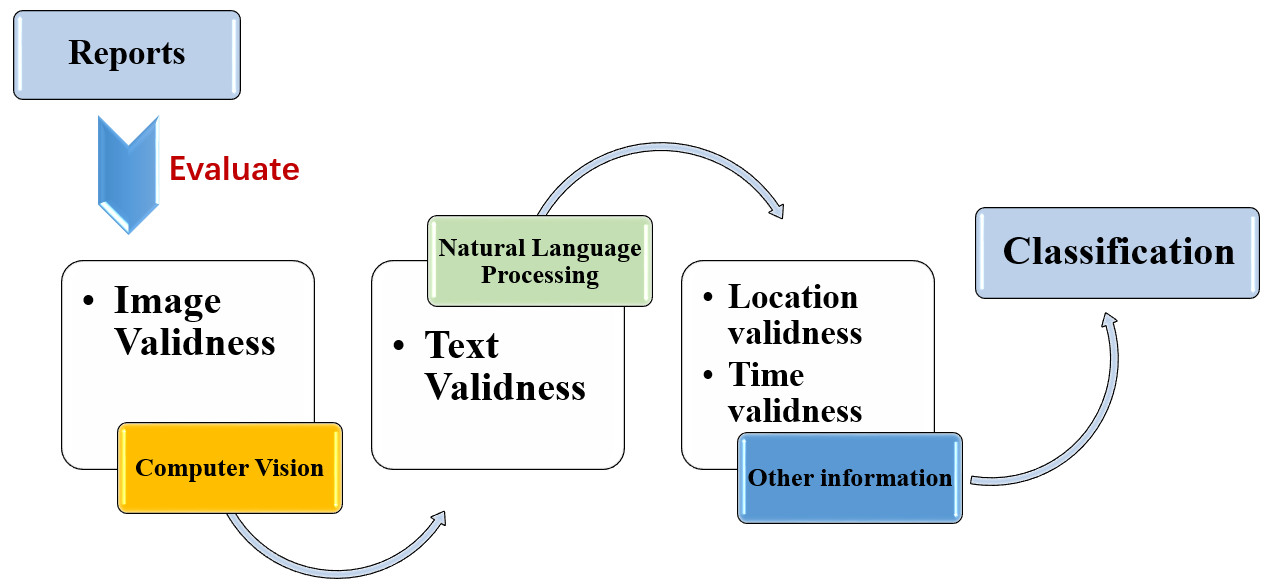
\includegraphics[scale=0.5]{procedure.png}
	\end{figure}\\
	Throughout the process of building the intelligent report classification model, we have accomplished several goals and obtain the following important results:
	\begin{enumerate}
		\item \textbf{The spread of the pest is predictable}\\
		Before we have the idea of the intelligent report classification, we first set up a scoring probability model to investigate whether the spread could be predicted or not, and the result is positive. Knowing the spread could be predicted provides us a sense that when  classifying or prioritizing reports, factors such as location and time difference could be related, this stands as the base of our model, that is multiple factor could influence the model at the same time.
		\item \textbf{Intelligent report classification model are able to predicts the likelihood of mistaken classification} \\
		With the aid of Computer Vision(CV) and Natural Language Processing (NLP), we are able to take both the images and the notes submitted along with the reports into consideration for our model. After using Analytic Hierarchy Process (AHP) to provide an evaluation function for our model, we successfully obtain the following function to score the reports for further operation:
		\begin{align*}
			L = 0.4772S_I + 0.2880S_T + 0.1539S_L + 0.0809S_D
			\label{final}
		\end{align*} 
		where $L$ represents the likelihood of a single report to be classified as "positive sightings"  and $S_I,S_T,S_I,S_D$ represents the four scores coming from Image,Text,Location and Time difference. Now that the evaluation(scoring) function has been defined, all we have to do to predict the likelihood of mistaken classification is to take the submitted report as input and rank them after obtaining their scores. Based on the frequency theory of probability, we set the last 50\% as the mistaken classification, and the estimated probability of a mistaken classification is 60.2\%.
		\item \textbf{Intelligent report classification model are able to provide the list of prioritized report}\\
		Since now we have the evaluation function, we are able to use our model to help the Washington State to prioritize the submitted reports. There is no doubt that there exists several reports that requires investigation in priority, therefore, after applying our model, we could rank all the reports and investigate the top 5\% report first. As a matter of fact, the precision of our model when prioritizing valuable reports is estimated as 78.6\%.
		\item \textbf{The model's update is a dynamic process}\\
		By no means a model could last eternally and benefit the user forever, so the intelligent report classification model requires to be updated, and the update progress would be in a dynamic form. First of all, the method of the update should cover the following four aspects: image(photos), text(notes), location and time difference. Second, the update frequency would be the dynamic result after taking both pest and human resources into account. We use the difference equation model to build up an estimated curve of Asian Hornet's population growth and in combination of the frequency curve of the submitted reports, we are able to design the following update frequency as presented in the figure.
		\begin{figure}[h]
			\centering
			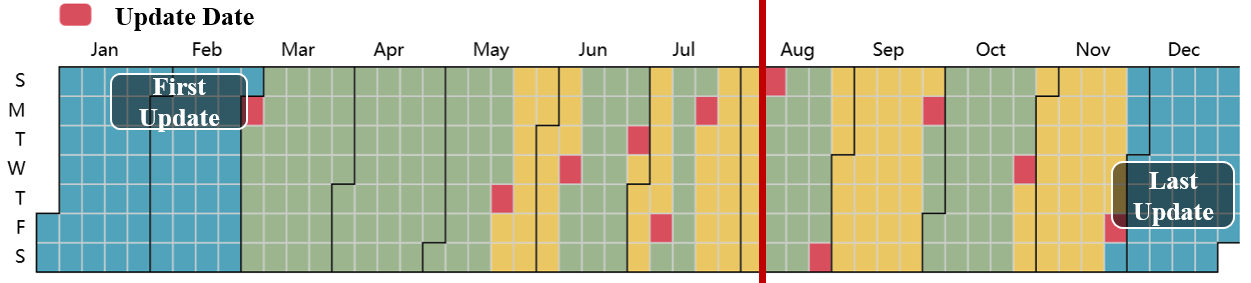
\includegraphics[scale=0.5]{calendar.png}
		\end{figure}
		\item \textbf{The indication of the pest's eradication could be realized }\\
		Our model is designed to inspect the pest and try to follow up with the control. After designing a model like this, we could also apply it to supervise the eradication process of Asian Hornet. After we prioritizing several reports in Spring and Winter and mark them on the map, we could decide whether they have been extinct or not based on the background information by drawing a circle of 30km and 8km to enclose them and count the number. Indeed, The indication of the pest's eradication could be realized
	\end{enumerate}
	\quad All the results we obtained are presented above, and hope the intelligent classification model we created could be a great use and help the Washington State overcome the obstacles eventually.
	\begin{flushright}
		Yours,\\
	Team\#2102416
	\end{flushright}
	
\newpage
\bibliographystyle{IEEETran}
%\bibliographystyle{plain}

\begin{thebibliography}{3}
\bibitem{intro0}Asian Giant Hornet, 2021MCM\_ProblemC\_Vespamandarina, PennState Extension.
\bibitem{intro1}Gallai N, Salles J-M, Settele J, Vaissiere BE (2009) Economic valuation of the vulnerability of world agriculture confronted with pollinator decline. Ecol Econ 68:810–821. doi:10.1016/j.ecolecon.2008.06.014
\bibitem{Task_1_1}Daniel N. Franklin, Mike A. Brown, Samik Datta, Andrew G. S. Cuthbertson, Giles E. Budge,Matt J. Keeling
\bibitem{Yolo}Redmon J, Farhadi A. Yolov3: An incremental improvement[J]. arXiv preprint arXiv:1804.02767, 2018.
\bibitem{Word}Goldberg Y, Levy O. word2vec Explained: deriving Mikolov et al.'s negative-sampling word-embedding method[J]. arXiv preprint arXiv:1402.3722, 2014.
\bibitem{LeNet}El-Sawy A, Hazem E L B, Loey M. CNN for handwritten arabic digits recognition based on LeNet-5[C]//International conference on advanced intelligent systems and informatics. Springer, Cham, 2016: 566-575.
\bibitem{reproduction} V.B.Wigglesworth,The Hormonal Regulation of Growth and Reproduction in Insects,Editor(s): J.W.L. Beament, J.E. Treherne, V.B. Wigglesworth,Advances in Insect Physiology,Academic Press,Volume 2,1964,Pages 247-336,ISSN 0065-2806,ISBN9780120242023,https://doi.org/10.1016/S0065-2806(08)60076-4.
\bibitem{functional_extinction} P.G. Javier; C. Vânia; S. Pedro; S. Jon; C. Juan; F.L. Pedro; Z. Attila; M.N. M.; A. István; B. József; V. Gyula; B. Albano (2014-12-26). "Males and Females Contribute Unequally to Offspring Genetic Diversity in the Polygynandrous Mating System of Wild Boar". PLOS ONE. 9 (12). e115394. 
\end{thebibliography}
\newpage


\end{document}


